\section{Designs for Secure Virtualization Systems}
\label{sec.design}

%Many security systems for protecting privileged code have been proposed and
%developed over the years. The challenge for all of these systems is how to
%balance security and functionality for applications. In this section, we explore previous approaches to
%dealing with this safety/usability trade-off.

A fundamental design question in a secure virtualization system
is how to provide essential system functionality.
There are two basic approaches.
One is to check and pass through system calls to the underlying kernel,
or ``System Call Interposition (SCI)."
The other is to rebuild system functionality with new code,
which we call ``functionality reimplementation."
In this section, we highlight the key ideas behind both designs, and
discuss their deficiencies in preventing attacks
%from triggering and exploiting vulnerabilities
in the kernel.
Lastly, inspired by the idea of ``functionality reimplementation,"
%but taking it a step further,
we present a third
alternative that ensures the safety of reimplementation through isolation
within a secure environment.

\subsection{System Call Interposition (SCI)}
SCI is the long-standing idea behind sandboxing systems like Janus
\cite{Janus0:96, Janus:99}. It relies on the underlying kernel
to provide system functionality. To prevent attackers from undermining the system,
SCI uses a system call filter module to mediate requests
from untrusted user code instead of allowing it to go directly to the kernel.
The filter will check a predefined security policy to decide which system calls are
allowed to pass to the underlying kernel, and which ones must be stopped.
%The security policy usually
%can be defined by the system administrator through a policy engine.
%
Figure \ref{fig:design_system_call_interposition} illustrates the general design
of a system call interposition system.

\begin{figure}%[h]
\centering
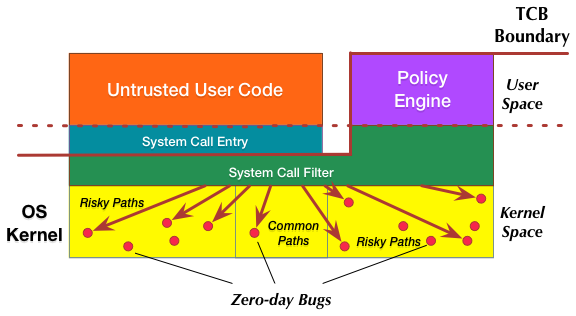
\includegraphics[width=1.0\columnwidth]{diagram/Virtualization_Design_Model_03.png}
\caption{\small System Call Interposition.}
\label{fig:design_system_call_interposition}
\end{figure}

System call interposition was once a popular approach to the design of secure
virtualization systems because it gave developers the power to set and enforce
security policies.
%that could pass or stop a system call in a straightforward way.
\lois{Does the use of the past tense here suggest
such an approach is no longer popular?}  However, this design
is limited by its overly complicated approach to policy decisions and implementation.
First, to make a policy decision, the system needs to
obtain and interpret the OS state associated with the programs it is monitoring.
The complexity of OS states makes this process difficult and can lead to
inaccurate policy decisions.
Second, there are many indirect paths in the kernel that can be accessed.
Overlooking those paths would render the
system call interposition policy ineffective, because attackers will be able to
bypass the imposed security checks. Moreover, many side-effects of blocking
certain system calls could affect the function of desired system calls.
It is difficult for developers to fully understand the side-effects of all the
system calls in an interface as complex as the UNIX API. This makes
it challenging to design and build a secure virtualization system using
system call interposition alone.
%Eventually, developers turned to the idea of
%reimplementation, which is more practical.

\subsection{Functionality Reimplementation}
Since using system call interposition alone is not sufficient,
%to serve the purpose of
%a modern system, where complex and risky system functionality is required,
many virtualization systems have created their own system
interface and library. Systems such as  Drawbridge \cite{Drawbridge-11},
 Bascule \cite{Bascule}, and Graphene \cite{Graphene-14} can
provide richer functionality and run complex programs. Some virtualization
systems, such as OS VM systems VirtualBox, and VMWare Workstation, even have the
full functionality of an OS reimplemented in their codebase. We call such a design
``Functionality reimplementation."


\begin{figure}%[h]
\centering
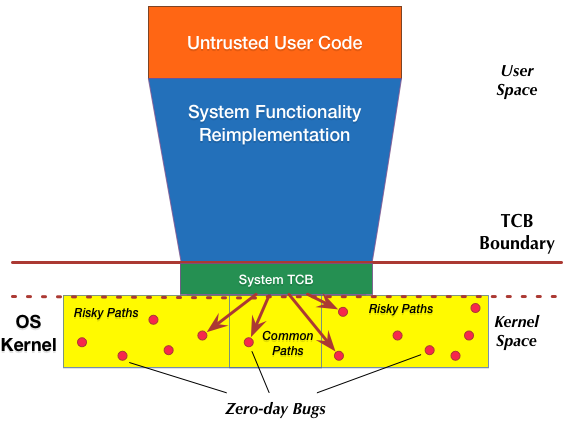
\includegraphics[width=1.0\columnwidth]{diagram/Virtualization_Design_Model_02.png}
\caption{\small Functionality reimplementation.}
\label{fig:design_functionality_reimplementation}
\end{figure}

The key idea of this design is to not fully rely on the underlying
kernel for system functions. Instead, essential OS functions are written with new
code. As illustrated in Figure \ref{fig:design_functionality_reimplementation},
in this design, the system will have its own system functionality reimplemented and
provided to the user code. When it has to communicate with the kernel
to access resources like memory, CPU, and disk storage, it will do so with
its underlying TCB code, which can access the kernel directly.
For example, Graphene \cite{Graphene-14} reimplements
its own Linux system calls in the
\texttt{libLinux.so} module. When it needs to acquire essential resources from
the kernel, it uses a
Platform Adaptation Layer (PAL)  module that has access to the kernel
and provides basic ABI functions to the OS library.

Functionality reimplementation provides a
realistic solution to building virtualization systems
with rich functionality. However, it
%is not as secure as people have thought and
leaves plenty of opportunities for attackers.\lois{Proof of this? Citations?}
First, to provide rich functions, systems using this design have
introduced larger codebases and increased the size of their TCBs.
The complexity of OS functions can easily result in bugs and vulnerabilities in
reimplementation. Some vulnerabilities
will directly cause a privilege escalation, which allows attackers to escape the sandbox
and execute arbitrary code on the host OS.
%Besides these severe vulnerabilities that can lead to attackers taking direct control
%of the machine,
Even operations that are considered
legal and harmless in the guest OS may open up system call paths into the underlying
host OS and cause a problem.
The second type of problem can be fatal, as it can reach and
trigger vulnerabilities in the underlying OS kernel.

%Problems with the existing functionality reimplementation design indicate that there
%is a lot more to do to build secure virtualization systems. The next step was to
%combine the strengths of both systems and the guidance of our metric to explore a
%new design template.

\subsection{Functionality Safe Reimplementation}
We propose a new design that adds additional security to
functionality reimplementation, by leveraging our key observation
 that "commonly used kernel paths contain fewer bugs"
(Section {\ref{sec.metric}).
The key to this design is that all code \emph{including the complex part
of the operating system interface} should have a very small TCB that accesses only
commonly used kernel paths. Any complex or possibly risky system functions
should be reimplemented using memory-safe code in a sandbox.
%In this manner, any bugs
%or failures within the implementation of these complex system functions
%are contained by the sandbox.
As a result, untrusted code would not be able to
trigger sensitive and risky portions of the kernel.
We call this design "functionality safely reimplementation,"
which provides extra security by combining reimplementation of
complex functionality with isolation and protection.

One approach to building such a system is to place it entirely in the userspace,
and restrict both the size of the sandbox kernel and its access to the
OS kernel (Figure \ref{fig:design_safe_reimplementation}).
This approach has advantages over others that require modifications to
the OS kernel.
%as it avoids the risk of threat escalation.
If a modified module is in the OS kernel and is compromised, it exposes
kernel privileges that could allow attacks
on the underlying system, as well as any applications running on top of it.

As shown in Figure \ref{fig:design_safe_reimplementation}, our secure virtualization system
has two components. First, as our secure system should support and run legacy applications,
and execute binary code compiled from unmodified source code on popular hardware architecture
like x86 architecture, it needs a computation module.
This module's main responsibility is providing an execution environment
that can run unmodified source code. It also performs functions like type checking,
object creation, and garbage collection.
The key security issue of executing system calls
without triggering OS kernel bugs is left to the second module, a library OS
that serves requests to access the OS kernel.
These two components can complete the requirements of running user code.
The system invokes the computation module to perform its operations,
and, if there are riskier calls, its computation module directs those requests to the
library OS. In turn, the library OS responds to the system call requests and
returns results to the user code, if the requests are granted.

\begin{figure}%[h]
\centering
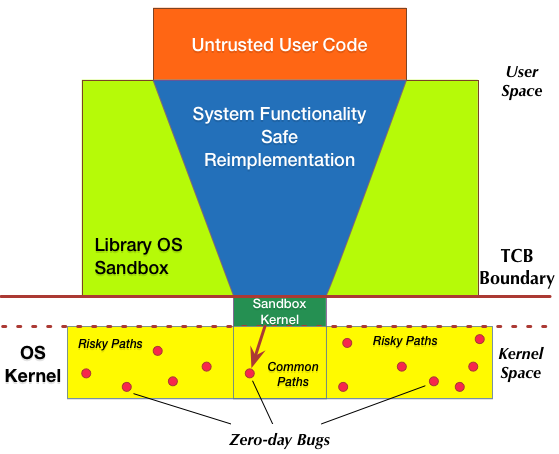
\includegraphics[width=1.0\columnwidth]{diagram/Virtualization_Design_Model_01.png}
\caption{\small ``Safe Reimplementation'' that ensures predictable execution of untrusted user code
despite existing potential zero-day bugs in the OS kernel.}
\label{fig:design_safe_reimplementation}
\end{figure}


%\subsubsection{The Computation Module}
%
%Providing an execution environment that can run unmodified source code is
%the main responsibility of the computation module. The key security issue of executing system calls
%without triggering OS kernel bugs is left to the library OS module.

%\subsubsection{The Library OS Module}

\textbf{The Library OS module} is the core of our virtualization system. It is comprised
of two parts: a sandbox kernel that provides access to basic but critical
system calls, and a system API safe reimplementation that implements more
complex calls, such as file system calls.

The sandbox kernel forms the only TCB of our library OS.
We make the kernel extremely small and simple so that it is easy to verify its security.
The sandbox code provides an API that performs
a few critical system calls with the most basic parameters, such as
writing data to the file system
and communicating with the network.  The kernel utilizes the most simplistic calls
possible with the most
basic arguments. In the example above, the file system API only need to provide a way
to write data to storage. \yanyan{where is the example?} It need not provide a directory abstraction, the
concept of file permissions, links, or even the concept of multiple files.

%It should have a set of capabilities that enable the construction of essential and more complicated functions.
%For example, the sandbox kernel capabilities should include basic functions for network,
%file system I/O, lock, thread, and namespace. It also needs to have access to the OS kernel through system calls.
%In developing our design, we leveraged our verified hypothesis that commonly used kernel paths contain fewer bugs.
%Thus, the system calls we allow in our sandbox kernel are common calls, like file open, read, write, and close.
%Furthermore, the set of arguments used for each call is also highly restricted.

The system API safe reimplementation is a set of more complicated system calls
derived from functions in the sandbox kernel.
We reimplement those system calls because we do not want this potentially risky user code
to have direct access to the underlying OS kernel.
Instead, our reimplementation layer serves as a mediator between the user code
and the OS kernel. The reimplementation is safe
because the reconstructed calls are isolated in a sandbox, and the code for the
reimplementation is written in a memory-safe programming language.

Here is an example of how this reimplementation would work with the symbolic link function.
If there is a bug in this function, rather than rely on the kernel code paths
for symbolic links, our sandbox system will implement the incorrect behavior.
This denies the code the privileged access to the system the OS kernel does.
As a result, instead of creating a security issue, the application will just fail.
\yanyan{this paragraph feels a bit weak. instead of blocking or denying, do
we do anything else?}

With the computation module and the library OS module, unmodified user code is able to run on top of our designed system.
It is important to note that our design does not rely on any specific technique or tool, and it is possible
to choose from several different techniques that fit well with the users' specific needs or requirements.
The following section describes one implementation of our design.

%Based on this general system, we implemented a prototype security system based on a controlled kernel access that we called Lind.
%Below we offer a short explanation of one design feature: the use of dual sandboxes.
%The following section offers a more detailed description of Lind's design and implementation.
%
%\subsection{The Roles of the Dual Sandboxes}
%
%In reviewing our design, some fundamental questions could be raised about the dual sandbox design choice.
%"Why is one not enough?"" And, "If two is good, why not use three or more?""
%The answer to the first question is that the kernel interface is extremely rich and hard to protect.
%In order to have minimal impact on the kernel, as well as provide sufficient API for legacy applications,
%we need to have one sandbox focuses on protecting the kernel and providing POSIX API.
%With two sandboxes, one serves as the computation module,
%while the other one is the library OS module. As to the second question,
%which could be rephrased as ``why not sandbox the sandbox kernel TCB and get more security?,''
%the lowest level sandbox eventually must have some fundamental,
%even if limited, access to system resources, such as memory, and storage, threads.
%So even if we were to sandbox the sandbox kernel and have additional sandboxes,
%the one at the bottom level will still access the OS kernel in a similar way.
%Thus, having multiple sandboxes does not provide any extra security benefits.
%\yanyan{it's better to tie in with earlier paragraphs and talk about why we need
%computation + lib OS. we normally don't do Q\&A like this.}
